\def\tightlist{}
\documentclass[signature, dutch, biblatex]{deltares_report}
% \bibliography{bib/westerscheldewillem,bib/library}
$if(highlighting-macros)$
$highlighting-macros$
$endif$
$if(csl-refs)$
% Pandoc citation processing
\newlength{\cslhangindent}
\setlength{\cslhangindent}{1.5em}
\newlength{\csllabelwidth}
\setlength{\csllabelwidth}{3em}
\newlength{\cslentryspacingunit} % times entry-spacing
\setlength{\cslentryspacingunit}{\parskip}
% for Pandoc 2.8 to 2.10.1
\newenvironment{cslreferences}%
 {$if(csl-hanging-indent)$\setlength{\parindent}{0pt}%
 \everypar{\setlength{\hangindent}{\cslhangindent}}\ignorespaces$endif$}%
 {\par}
% For Pandoc 2.11+
\newenvironment{CSLReferences}[2] % #1 hanging-ident, #2 entry spacing
 {% don't indent paragraphs
  \setlength{\parindent}{0pt}
  % turn on hanging indent if param 1 is 1
  \ifodd #1
  \let\oldpar\par
  \def\par{\hangindent=\cslhangindent\oldpar}
  \fi
  % set entry spacing
  \setlength{\parskip}{#2\cslentryspacingunit}
 }%
 {}
\usepackage{calc}
\newcommand{\CSLBlock}[1]{#1\hfill\break}
\newcommand{\CSLLeftMargin}[1]{\parbox[t]{\csllabelwidth}{#1}}
\newcommand{\CSLRightInline}[1]{\parbox[t]{\linewidth - \csllabelwidth}{#1}\break}
\newcommand{\CSLIndent}[1]{\hspace{\cslhangindent}#1}
\renewcommand{\FrontCover}{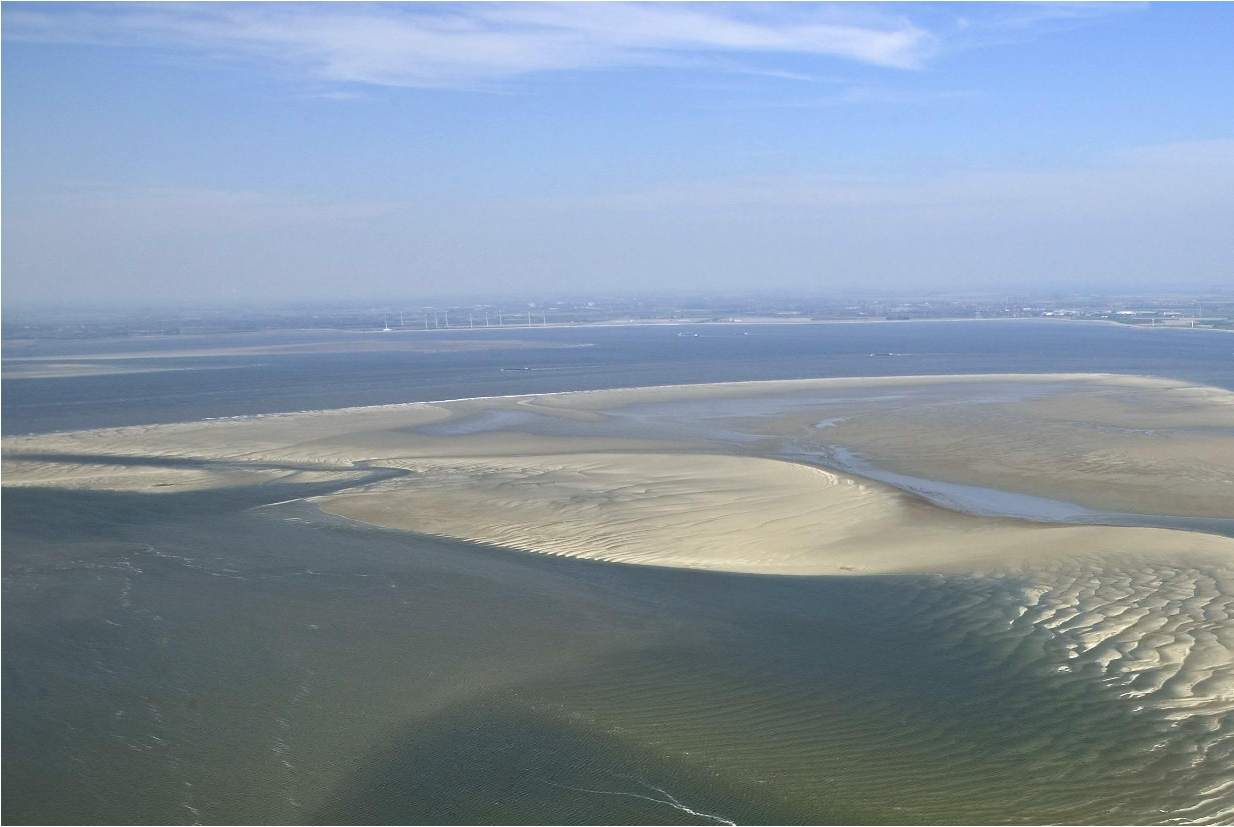
\includegraphics[width=182mm,height=182mm]
{Figuren/cover/getijdenland.pdf}}
\coverPhoto{}
$endif$
\begin{document}
\title{Eerstelijn Rapportage Westerschelde}
\subtitle{1998 - 2022}
\author{W. Stolte, J. Rienstra}
\partner{}

\client{Rijkswaterstaat WVL, VNSC}
\contact{Albert Mulder}
\reference{}
\keywords{hydrodynamiek, waterkwaliteit, zwevend stof, sediment, biota, fytoplankton}

\version{2023}
\date{03-12-2023}
\projectnumber{1209394}
\documentid{}
\status{definitief}
\disclaimer{}
% \references{References}

\authori{Willem Stolte, Jelle Rienstra}
\organisationi{Deltares}
\versioni{1.0}
\datei{03-12-2023}
\revieweri{Arno Nolte}
\approvali{Toon Segeren}
\publisheri{Deltares}

\summary{
Deze rapportage is opgemaakt met door RWS in de Scheldemonitor beschikbaar gemaakte hydrodynamische, fysisch-chemische en biologische gegevens (alleen fytoplankton). De rapportage gaat over gegevens verzameld in de periode 1996 tot en met `r dataJaar` voor de Westerschelde en de monding. De gegevens zijn verkregen in het kader van de Nederlandse MWTL monitoring. Het is een eerste weergave van de beschikbare data en heeft als doel om enkel te beschrijven ‘wat men in de meetresultaten ziet’. Het bevat een korte interpretatie van de gegevens op basis van een eenvoudige analyse. 

De rapportage is opgesteld in het kader van de OntwikkelingsSchets 2010 en vormt een van de bouwstenen voor de vergunningverlening van de derde verdieping van het Schelde-estuarium. 

De verdere duiding van deze en Vlaamse gegevens wordt gedaan in de 6-jarige cyclus van analyse- en eveluatierapportage, de zogenaamde T-rapportages. Aangezien deze analyse- en evaluaties een vastgestelde methodiek volgen van waaruit verdere gevolgtrekkingen wordt gedaan, wordt in deze eerstelijnsrapportage verder geen duiding gegeven aan de resultaten. 

}
\deltarestitle
%------------------------------------------------------------------------------

% Text body

$body$

%------------------------------------------------------------------------------
\end{document}
